\documentclass[12pt]{article}
\usepackage{amsmath}
\usepackage{listings}
\usepackage{textcomp}
\usepackage{graphicx}
\usepackage[utf8]{inputenc} % allow utf-8 input
\usepackage[T1]{fontenc}    % use 8-bit T1 fonts
\usepackage{hyperref}       % hyperlinks
\usepackage{url}            % simple URL typesetting
\usepackage{booktabs}       % professional-quality tables
\usepackage{amsfonts}       % blackboard math symbols
\usepackage{nicefrac}       % compact symbols for 1/2, etc.
\usepackage{microtype}      % microtypography
\setlength{\parindent}{0pt}

\graphicspath{{./fig/}}

\newcommand{\skipline}{\vspace{\baselineskip}}

\begin{document}

\textit{Github: github.com/3tz/Jester-Online-Jokes-Analysis}

\section{Pre-processing}

  \subsection{Matrix Transformation}

    \quad First, all datasets are transformed into a matrix with each row containing one single rating and the columns of this matrix containing user IDs, item IDs, and ratings. Here, a user ID is the ID number of the person who rates the jokes and item ID is the ID number of the joke. To use Non-negative Matrix Factorization (NMF), all ratings must be non-negative. Thus, the ratings in the matrix are simply shifted to the positive direction by a value of 10. For Multilayer Perceptron model (MLP), the ratings are shifted back with the center being 0. Below is a summary of the matrix with an extra column of "nRated" which is just the number of jokes this person has rated for the purpose of organizing; only the first three columns of the matrix will be used for training. Notice that this matrix is a full matrix with no missing value.

    \lstset{language = R, upquote=true}
    \begin{lstlisting}[basicstyle=\small\tt, numbers=left]
           uID jID rating nRated
      1:     1   1   2.18     74
      2:     1   2  18.79     74
      3:     1   3   0.34     74
      4:     1   4   1.84     74
      5:     1   5   2.48     74
     ---
4136356: 73421  65  11.36     35
4136357: 73421  66  17.18     35
4136358: 73421  69  10.49     35
4136359: 73421  72  15.87     35
4136360: 73421  82  16.65     35
    \end{lstlisting}

  \subsection{Cross Validation}

    \quad Recommender systems, especially non-negative matrix factorization, should not encounter new user or item ID during prediction that the models have not yet encountered during training. Thus, to achieve the goal of predicting ratings of all 100 jokes for every pre-selected 300 users, we will have multiple pairs of training and testing sets to guarantee mutual-exclusiveness. For instance, for a training set with a size of 30$\%$ of the total data, pseudocode of the operation is the following:

    \skipline

    \lstset{language = Python, upquote=true}
    \begin{lstlisting}[basicstyle=\footnotesize, numbers=left]
for i in allUserIDs:
  pair1_trainSet.append(30 random ratings from user i)
    if i is one of the 300 testing users:
      pair1_testSet.append(remaining 70 jokes from user i)
    pair2_trainSet.append(30 random ratings from pair1_testSet)
pair2_testSet = ratings rated by the 300 users in pair1_trainSet
    \end{lstlisting}



    \quad This algorithm follows three rules: training set in each pair contains only the specified percentage of the total dataset, the union of test sets from all pairs cover all of the joke IDs, and user IDs in the training set are guaranteed to not exist in the testing set for each pair. Thus, if there were only 10 joke IDs, for a user who is one of the 300 testing users, assignments of joke IDs of ratings would look like this:

    \lstset{language = R, upquote=true}
    \begin{lstlisting}[basicstyle=\small\tt]
       trainSetJokeIDs  testSetJokeIDs
pair1: [1,2,3]          [4,5,6,7,8,9,10]
pair2: [4,5,9]          [1,2,3]
    \end{lstlisting}

    where \texttt{[1,2,3]} are first randomly chosen from 1 to 10, and \texttt{[4,5,9]} are randomly chosen from \texttt{[4,5,6,7,8,9,10]}. Notice that we indeed only contain 30$\%$ of the dataset for training, the union of test sets from all pairs contains each testing joke ID once, and user IDs in the training set are guaranteed to not exist in the testing set for each pair.

    \quad For a training set with a size of higher than 50$\%$ of the total data, a similar strategy is used but with more pairs of training and testing sets. For instance for a training set with a size of $60\%$ of the total data, 3 pairs of training and testing sets are required, and joke assignments to datasets would look like this for one of the user in the testing set (IDs during actual operations are randomly chosen; they are in numerical order for demonstration purpose):

    \lstset{language = R, upquote=true}
    \begin{lstlisting}[basicstyle=\small\tt]
       trainSetJokeIDs  testSetJokeIDs
pair1: [1,2,3,4,5,6]    [8,9,10]
pair2: [1,2,3,8,9,10]   [4,5,6,7]
pair3: [4,5,6,7,8,9]    [1,2,3]
    \end{lstlisting}

    \quad The same three rules are also followed.

\newpage \section{Result}

  \subsection{Non-negative Matrix Factorization}

    \subsubsection{MAE}

      \begin{center}
        \textit{Training MAE} \qquad \qquad \qquad \quad \textit{Validation MAE}

        \begin{tabular}{|l || l| l| l|}
          \hline
          &\multicolumn{3}{|c|}{Training Size} \\
          %\cline{2-4}
          \hline
          Rank & 30\% & 60\% & 90\% \\
          \hline
          1 & 3.342 & 3.398 & 3.418 \\
          10 & 2.559 & 2.802 & 2.879 \\
          20 & 2.001 & 2.438 & 2.599 \\
          30 & 1.665 & 2.181 & 2.392 \\
          40 & 1.442 & 1.970 & 2.223 \\
          50 & 1.246 & 1.796 & 2.068 \\
          60 & 1.136 & 1.671 & 1.956 \\
          70 & 1.047 & 1.558 & 1.860 \\
          80 & 0.976 & 1.479 & 1.776 \\
          90 & 0.914 & 1.385 & 1.688 \\
          100 & 0.878 & 1.321 & 1.622 \\
          150 & & & 1.393 \\
          200 & & & 1.255 \\
          250 & & & 1.170 \\
          300 & & & 1.114 \\
          350 & & & 1.075 \\
          \hline
        \end{tabular}
        \begin{tabular}{|l || l| l| l|}
          \hline
          &\multicolumn{3}{|c|}{Training Size} \\
          %\cline{2-4}
          \hline
          Rank & 30\% & 60\% & 90\% \\
          \hline
          1   & 3.684 & 3.664 & 3.648 \\
          10  & \underline{\textbf{3.537}} & 3.354 & 3.303 \\
          20  & 3.574 & \underline{\textbf{3.339}} & 3.278 \\
          30  & 3.631 & 3.377 & \underline{\textbf{3.266}} \\
          40  & 3.616 & 3.364 & 3.268 \\
          50  & 3.629 & 3.383 & 3.269 \\
          60  & 3.610 & 3.386 & 3.275 \\
          70  & 3.606 & 3.372 & 3.275 \\
          80  & 3.595 & 3.382 & 3.277 \\
          90  & 3.600 & 3.387 & 3.282 \\
          100 & 3.577 & 3.375 & 3.277 \\
          150 & & & 3.280 \\
          200 & & & 3.288 \\
          250 & & & 3.274 \\
          300 & & & 3.278 \\
          350 & & & 3.281 \\
          \hline
        \end{tabular}

        \skipline

        \textit{Note: The lowest validation MAE for each training size is underlined.}
      \end{center}


      \begin{center}
        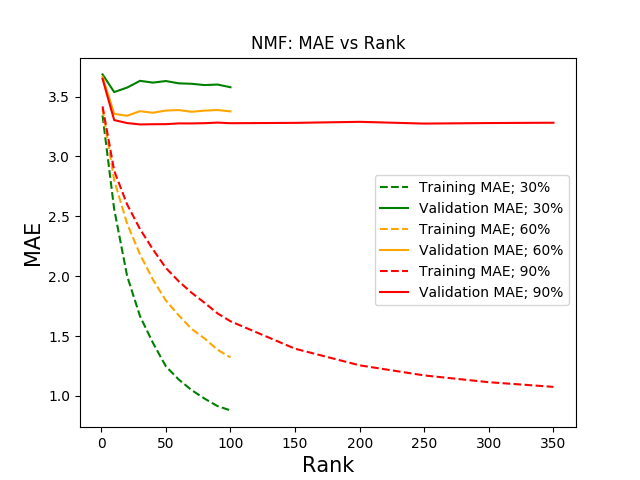
\includegraphics[scale=0.75]{nmf_mae.png}
      \end{center}

      \quad The MAE of the training set is calculated in the following way where $n$ denotes the number of pairs, $\hat{y}$ denotes vector containing the predicted values, and $y$ denotes the vector containing the true values. The superscript indicates the pair index and the subscript indicates the item in the vector.

      $$
      \frac{1}{n} \frac{1}{size(y)} \sum_{i=1}^{n} \sum_{j=1}^{size(y)} | \hat{y}_{j}^{(i)} - y_{j}^{(i)}|
      $$

      \quad Since MAE of the testing set is calculated after combining the predicted values together, the predicted values here are simply the $300 \times 100$ ratings in the pre-selected testing set. Thus, the MAE is simply

      $$\frac{1}{size(y)} \sum_{j=1}^{size(y)} | \hat{y}_{j} - y_{j}|$$.


    % \newpage\subsubsection{Ternary Compaison Against Baseline}
    %     \begin{center}
    %       \textit{Proportion of each ternary with each training size's optimal rank.}
    %
    %       \begin{tabular}{| c || c| c | c|}
    %         \hline
    %         &\multicolumn{3}{c|}{Ternary Proportion} \\
    %         \hline
    %         Model & a & b & c \\
    %         \hline
    %         NMF (90\%) & 55.300\%  & 29.640\% & 15.060\% \\
    %         NMF (60\%) & 54.523\%  & 29.647\% & 15.830\% \\
    %         NMF (30\%) & 51.253\%  & 30.703\% & 18.043\% \\
    %         \hline
    %         Total Average & 14.257\% & 11.180\% & 74.563\% \\
    %         Uniformly Random & 12.720\% & 13.560\% & 73.720\% \\
    %         User Average &  8.463\% & 12.283\% & 79.253\% \\
    %         \hline
    %       \end{tabular}
    %
    %       \textit{Note: a: MAE $\in (-\infty ,3)$; b: MAE $\in [3 ,6)$; c: MAE $\in [6 ,\infty)$.}
    %
    %     \end{center}

  \newpage\subsection{Multilayer Perceptron}

    \subsubsection{Model Structure}
    \quad

    \begin{center}
      \textit{Visual Model Overview}

      \skipline

      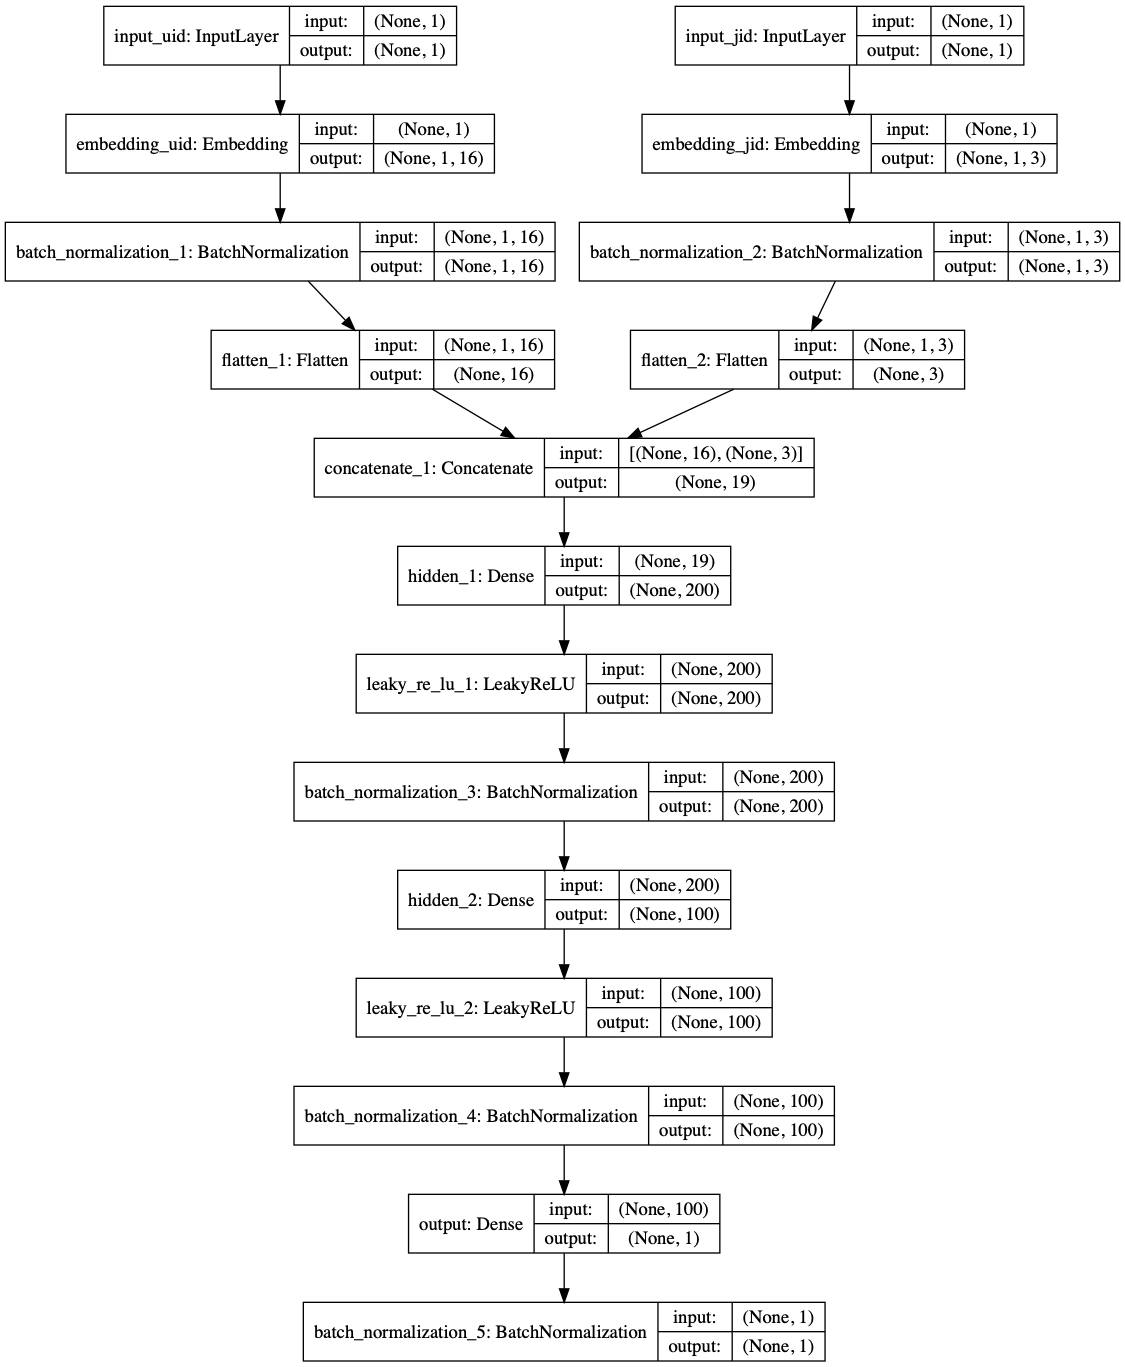
\includegraphics[width=0.8\textwidth]{model_plot.png}
    \end{center}

    \quad The loss function and the optimizer of the network are mean squared error and Adam with a learning rate of 0.1, and a batch size of 4096 is used for training.

    \quad The architecture of the layers follows the structure discussed by He \textit{et al} in his paper published in 2017[1]. This model takes two scalar inputs: user ID and joke ID. Then, each scalar input is fed into a different embedding layer. The idea of embedding was first introduced in the field of Natural Language Processing by Bengio \textit{et al}[2]. The purpose of an embedding layer is to reduce the high dimensionality of high cardinality discrete variable representation into a much smaller vector space. Here, the embedding layers convert each input into a vector of length 16 and 3 for user ID and joke ID which have a cardinality of $73,421$ and $100$ respectively, and the length of each vector is computed by taking the fourth root of the cardinality of the input. The way the IDs are converted into vectors is by assigning one vector of numerical values to every unique ID. The numerical values in these embedding vectors are initialized uniformly randomly and are updated during backpropagation based on the network's loss function in the same way as other layers' weights. Then, each of the vectors is normalized with Batch Normalization, and the normalized outputs are flattened and concatenated together as one single layer which is then fed to the hidden layers.

    \quad There are two hidden layers where the first layer contains 200 neurons and the second contains 100 neurons. Both of them are fully connected layers, have Leaky ReLU as their activations, and are normalized with Batch Normalization. The output layer has a size of one and a linear function as its activation, and its output is also normalized with Batch Normalization. Layer dropout is not used as it interferes with Batch Normalization which reduces performance when these two techniques are used together as discussed in [3].

    \newpage\subsubsection{MAE}

        \begin{center}
          \textit{Training MAE}

          \tiny
          \begin{tabular}{|l || l| l| l|}
            \hline
            &\multicolumn{3}{|c|}{Training Size} \\
            %\cline{2-4}
            \hline
            Epoch & 30\% & 60\% & 90\% \\
            \hline
            1 & 3.755 & 3.619 & 3.554 \\
            2 & 3.385 & 3.337 & 3.301 \\
            3 & 3.250 & 3.214 & 3.177 \\
            4 & 3.132 & 3.109 & 3.073 \\
            5 & 3.019 & 3.012 & 2.994 \\
            6 & 2.917 & 2.928 & 2.930 \\
            7 & 2.823 & 2.854 & 2.876 \\
            8 & 2.729 & 2.789 & 2.829 \\
            9 & 2.635 & 2.729 & 2.788 \\
            10 & 2.547 & 2.675 & 2.752 \\
            11 & 2.463 & 2.626 & 2.721 \\
            12 & 2.385 & 2.583 & 2.693 \\
            13 & 2.317 & 2.544 & 2.669 \\
            14 & 2.254 & 2.509 & 2.646 \\
            15 & 2.200 & 2.478 & 2.627 \\
            16 & 2.148 & 2.450 & 2.609 \\
            17 & 2.102 & 2.424 & 2.592 \\
            18 & 2.057 & 2.401 & 2.577 \\
            19 & 2.014 & 2.379 & 2.563 \\
            20 & 1.981 & 2.360 & 2.551 \\
            21 & 1.944 & 2.343 & 2.539 \\
            22 & 1.910 & 2.325 & 2.528 \\
            23 & 1.880 & 2.310 & 2.518 \\
            24 & 1.856 & 2.296 & 2.509 \\
            25 & 1.832 & 2.281 & 2.500 \\
            26 & 1.812 & 2.270 & 2.492 \\
            27 & 1.789 & 2.258 & 2.484 \\
            28 & 1.769 & 2.246 & 2.476 \\
            29 & 1.750 & 2.235 & 2.469 \\
            30 & 1.735 & 2.225 & 2.463 \\
            31 & 1.718 & 2.216 & 2.457 \\
            32 & 1.705 & 2.208 & 2.451 \\
            33 & 1.688 & 2.199 & 2.445 \\
            34 & 1.675 & 2.191 & 2.440 \\
            35 & 1.663 & 2.181 & 2.435 \\
            36 & 1.654 & 2.175 & 2.430 \\
            37 & 1.643 & 2.168 & 2.425 \\
            38 & 1.631 & 2.161 & 2.421 \\
            39 & 1.626 & 2.155 & 2.417 \\
            40 & 1.616 & 2.149 & 2.412 \\
            41 & 1.607 & 2.144 & 2.408 \\
            42 & 1.594 & 2.137 & 2.405 \\
            43 & 1.589 & 2.133 & 2.401 \\
            44 & 1.580 & 2.127 & 2.397 \\
            45 & 1.575 & 2.121 & 2.394 \\
            46 & 1.570 & 2.116 & 2.391 \\
            47 & 1.557 & 2.110 & 2.388 \\
            48 & 1.553 & 2.106 & 2.385 \\
            49 & 1.545 & 2.104 & 2.382 \\
            50 & 1.534 & 2.098 & 2.379 \\
            \hline
          \end{tabular}
          \begin{tabular}{|l || l| l| l|}
            \hline
            &\multicolumn{3}{|c|}{Training Size} \\
            \hline
            Epoch & 30\% & 60\% & 90\% \\
            \hline
            51 & 1.533 & 2.094 & 2.376 \\
            52 & 1.529 & 2.091 & 2.373 \\
            53 & 1.517 & 2.086 & 2.371 \\
            54 & 1.516 & 2.083 & 2.368 \\
            55 & 1.513 & 2.079 & 2.366 \\
            56 & 1.506 & 2.076 & 2.363 \\
            57 & 1.496 & 2.072 & 2.361 \\
            58 & 1.499 & 2.068 & 2.359 \\
            59 & 1.490 & 2.064 & 2.356 \\
            60 & 1.481 & 2.064 & 2.354 \\
            61 & 1.483 & 2.059 & 2.352 \\
            62 & 1.480 & 2.056 & 2.350 \\
            63 & 1.475 & 2.053 & 2.348 \\
            64 & 1.471 & 2.051 & 2.346 \\
            65 & 1.468 & 2.049 & 2.344 \\
            66 & 1.462 & 2.046 & 2.342 \\
            67 & 1.459 & 2.043 & 2.340 \\
            68 & 1.455 & 2.040 & 2.338 \\
            69 & 1.453 & 2.036 & 2.336 \\
            70 & 1.450 & 2.035 & 2.335 \\
            71 & 1.448 & 2.034 & 2.333 \\
            72 & 1.446 & 2.030 & 2.331 \\
            73 & 1.440 & 2.027 & 2.330 \\
            74 & 1.436 & 2.026 & 2.328 \\
            75 & 1.433 & 2.025 & 2.326 \\
            76 & 1.430 & 2.022 & 2.325 \\
            77 & 1.423 & 2.019 & 2.323 \\
            78 & 1.426 & 2.018 & 2.322 \\
            79 & 1.421 & 2.015 & 2.320 \\
            80 & 1.417 & 2.013 & 2.319 \\
            81 & 1.417 & 2.010 & 2.318 \\
            82 & 1.413 & 2.010 & 2.316 \\
            83 & 1.415 & 2.007 & 2.315 \\
            84 & 1.409 & 2.005 & 2.314 \\
            85 & 1.408 & 2.003 & 2.312 \\
            86 & 1.409 & 2.002 & 2.310 \\
            87 & 1.401 & 2.000 & 2.309 \\
            88 & 1.400 & 1.999 & 2.308 \\
            89 & 1.402 & 1.998 & 2.307 \\
            90 & 1.392 & 1.995 & 2.306 \\
            91 & 1.397 & 1.994 & 2.305 \\
            92 & 1.391 & 1.993 & 2.303 \\
            93 & 1.390 & 1.990 & 2.302 \\
            94 & 1.387 & 1.989 & 2.301 \\
            95 & 1.383 & 1.988 & 2.300 \\
            96 & 1.381 & 1.987 & 2.299 \\
            97 & 1.381 & 1.984 & 2.298 \\
            98 & 1.381 & 1.985 & 2.297 \\
            99 & 1.383 & 1.982 & 2.296 \\
            100 & 1.373 & 1.980 & 2.295 \\
            \hline
          \end{tabular}
          \begin{tabular}{|l || l| l| l|}
            \hline
            &\multicolumn{3}{|c|}{Training Size} \\
            \hline
            Epoch & 30\% & 60\% & 90\% \\
            \hline
            101 & & & 2.294 \\
            102 & & & 2.293 \\
            103 & & & 2.292 \\
            104 & & & 2.291 \\
            105 & & & 2.290 \\
            106 & & & 2.289 \\
            107 & & & 2.288 \\
            108 & & & 2.287 \\
            109 & & & 2.286 \\
            110 & & & 2.285 \\
            111 & & & 2.284 \\
            112 & & & 2.283 \\
            113 & & & 2.282 \\
            114 & & & 2.282 \\
            115 & & & 2.281 \\
            116 & & & 2.280 \\
            117 & & & 2.279 \\
            118 & & & 2.278 \\
            119 & & & 2.278 \\
            120 & & & 2.277 \\
            121 & & & 2.276 \\
            122 & & & 2.275 \\
            123 & & & 2.275 \\
            124 & & & 2.274 \\
            125 & & & 2.273 \\
            126 & & & 2.272 \\
            127 & & & 2.271 \\
            128 & & & 2.271 \\
            129 & & & 2.270 \\
            130 & & & 2.269 \\
            131 & & & 2.268 \\
            132 & & & 2.268 \\
            133 & & & 2.267 \\
            134 & & & 2.266 \\
            135 & & & 2.266 \\
            136 & & & 2.265 \\
            137 & & & 2.265 \\
            138 & & & 2.264 \\
            139 & & & 2.263 \\
            140 & & & 2.263 \\
            141 & & & 2.262 \\
            142 & & & 2.261 \\
            143 & & & 2.261 \\
            144 & & & 2.260 \\
            145 & & & 2.259 \\
            146 & & & 2.259 \\
            147 & & & 2.258 \\
            148 & & & 2.258 \\
            149 & & & 2.257 \\
            150 & & & 2.257 \\
            \hline
          \end{tabular}
          \normalsize
          \newpage
          \textit{Validation MAE}

          \tiny
          \begin{tabular}{|l || l| l| l|}
            \hline
            &\multicolumn{3}{|c|}{Training Size} \\
            \hline
            Epoch & 30\% & 60\% & 90\% \\
            \hline
            1 & 3.778 & 3.579 & 3.535 \\
            2 & 3.622 & 3.499 & 3.475 \\
            3 & 3.574 & 3.471 & 3.403 \\
            4 & 3.559 & 3.443 & 3.367 \\
            5 & 3.588 & 3.412 & 3.346 \\
            6 & \underline{\textbf{3.547}} & 3.432 & 3.339 \\
            7 & 3.567 & \underline{\textbf{3.401}} & 3.343 \\
            8 & 3.588 & 3.407 & \underline{\textbf{3.338}} \\
            9 & 3.595 & 3.419 & 3.340 \\
            10 & 3.634 & 3.410 & 3.354 \\
            11 & 3.650 & 3.430 & 3.361 \\
            12 & 3.694 & 3.449 & 3.364 \\
            13 & 3.738 & 3.456 & 3.371 \\
            14 & 3.742 & 3.461 & 3.380 \\
            15 & 3.744 & 3.513 & 3.375 \\
            16 & 3.827 & 3.500 & 3.382 \\
            17 & 3.826 & 3.499 & 3.383 \\
            18 & 3.832 & 3.527 & 3.385 \\
            19 & 3.873 & 3.539 & 3.390 \\
            20 & 3.932 & 3.523 & 3.395 \\
            21 & 3.924 & 3.549 & 3.413 \\
            22 & 3.957 & 3.579 & 3.410 \\
            23 & 3.968 & 3.563 & 3.417 \\
            24 & 3.966 & 3.596 & 3.418 \\
            25 & 4.076 & 3.566 & 3.421 \\
            26 & 4.020 & 3.620 & 3.423 \\
            27 & 4.068 & 3.599 & 3.427 \\
            28 & 4.059 & 3.599 & 3.438 \\
            29 & 4.056 & 3.601 & 3.435 \\
            30 & 4.080 & 3.605 & 3.441 \\
            31 & 4.082 & 3.614 & 3.448 \\
            32 & 4.100 & 3.632 & 3.450 \\
            33 & 4.119 & 3.651 & 3.457 \\
            34 & 4.163 & 3.653 & 3.455 \\
            35 & 4.146 & 3.654 & 3.451 \\
            36 & 4.138 & 3.652 & 3.464 \\
            37 & 4.165 & 3.645 & 3.462 \\
            38 & 4.167 & 3.659 & 3.464 \\
            39 & 4.205 & 3.650 & 3.465 \\
            40 & 4.204 & 3.692 & 3.469 \\
            41 & 4.193 & 3.667 & 3.486 \\
            42 & 4.221 & 3.661 & 3.474 \\
            43 & 4.215 & 3.684 & 3.475 \\
            44 & 4.225 & 3.679 & 3.484 \\
            45 & 4.224 & 3.704 & 3.486 \\
            46 & 4.250 & 3.680 & 3.486 \\
            47 & 4.265 & 3.724 & 3.482 \\
            48 & 4.255 & 3.700 & 3.489 \\
            49 & 4.310 & 3.721 & 3.491 \\
            50 & 4.282 & 3.706 & 3.490 \\
            \hline
          \end{tabular}
          \begin{tabular}{|l || l| l| l|}
            \hline
            &\multicolumn{3}{|c|}{Training Size} \\
            \hline
            Epoch & 30\% & 60\% & 90\% \\
            \hline
            51 & 4.318 & 3.710 & 3.495 \\
            52 & 4.331 & 3.724 & 3.503 \\
            53 & 4.313 & 3.697 & 3.501 \\
            54 & 4.307 & 3.725 & 3.500 \\
            55 & 4.290 & 3.720 & 3.504 \\
            56 & 4.297 & 3.722 & 3.504 \\
            57 & 4.320 & 3.738 & 3.509 \\
            58 & 4.308 & 3.734 & 3.509 \\
            59 & 4.348 & 3.739 & 3.508 \\
            60 & 4.336 & 3.726 & 3.514 \\
            61 & 4.345 & 3.726 & 3.510 \\
            62 & 4.340 & 3.735 & 3.510 \\
            63 & 4.350 & 3.729 & 3.514 \\
            64 & 4.385 & 3.755 & 3.518 \\
            65 & 4.397 & 3.737 & 3.513 \\
            66 & 4.361 & 3.755 & 3.523 \\
            67 & 4.381 & 3.742 & 3.519 \\
            68 & 4.364 & 3.734 & 3.526 \\
            69 & 4.386 & 3.764 & 3.521 \\
            70 & 4.365 & 3.744 & 3.521 \\
            71 & 4.389 & 3.743 & 3.523 \\
            72 & 4.376 & 3.752 & 3.530 \\
            73 & 4.376 & 3.747 & 3.526 \\
            74 & 4.404 & 3.779 & 3.533 \\
            75 & 4.384 & 3.756 & 3.528 \\
            76 & 4.430 & 3.774 & 3.531 \\
            77 & 4.380 & 3.753 & 3.534 \\
            78 & 4.392 & 3.791 & 3.526 \\
            79 & 4.408 & 3.753 & 3.533 \\
            80 & 4.402 & 3.801 & 3.536 \\
            81 & 4.440 & 3.777 & 3.534 \\
            82 & 4.414 & 3.775 & 3.532 \\
            83 & 4.427 & 3.783 & 3.534 \\
            84 & 4.419 & 3.780 & 3.540 \\
            85 & 4.412 & 3.779 & 3.537 \\
            86 & 4.419 & 3.775 & 3.539 \\
            87 & 4.412 & 3.781 & 3.543 \\
            88 & 4.419 & 3.786 & 3.541 \\
            89 & 4.427 & 3.785 & 3.540 \\
            90 & 4.435 & 3.795 & 3.541 \\
            91 & 4.438 & 3.811 & 3.544 \\
            92 & 4.445 & 3.784 & 3.545 \\
            93 & 4.442 & 3.783 & 3.550 \\
            94 & 4.434 & 3.808 & 3.547 \\
            95 & 4.450 & 3.789 & 3.543 \\
            96 & 4.458 & 3.789 & 3.550 \\
            97 & 4.488 & 3.784 & 3.548 \\
            98 & 4.465 & 3.803 & 3.552 \\
            99 & 4.457 & 3.806 & 3.549 \\
            100 & 4.487 & 3.808 & 3.555 \\
            \hline
          \end{tabular}
          \begin{tabular}{|l || l| l| l|}
            \hline
            &\multicolumn{3}{|c|}{Training Size} \\
            \hline
            Epoch & 30\% & 60\% & 90\% \\
            \hline
            101 & & & 3.556 \\
            102 & & & 3.553 \\
            103 & & & 3.556 \\
            104 & & & 3.553 \\
            105 & & & 3.562 \\
            106 & & & 3.557 \\
            107 & & & 3.560 \\
            108 & & & 3.560 \\
            109 & & & 3.555 \\
            110 & & & 3.568 \\
            111 & & & 3.558 \\
            112 & & & 3.561 \\
            113 & & & 3.563 \\
            114 & & & 3.562 \\
            115 & & & 3.564 \\
            116 & & & 3.564 \\
            117 & & & 3.566 \\
            118 & & & 3.568 \\
            119 & & & 3.567 \\
            120 & & & 3.563 \\
            121 & & & 3.574 \\
            122 & & & 3.571 \\
            123 & & & 3.568 \\
            124 & & & 3.564 \\
            125 & & & 3.573 \\
            126 & & & 3.566 \\
            127 & & & 3.569 \\
            128 & & & 3.573 \\
            129 & & & 3.572 \\
            130 & & & 3.569 \\
            131 & & & 3.574 \\
            132 & & & 3.570 \\
            133 & & & 3.577 \\
            134 & & & 3.576 \\
            135 & & & 3.571 \\
            136 & & & 3.574 \\
            137 & & & 3.579 \\
            138 & & & 3.576 \\
            139 & & & 3.575 \\
            140 & & & 3.578 \\
            141 & & & 3.575 \\
            142 & & & 3.584 \\
            143 & & & 3.580 \\
            144 & & & 3.581 \\
            145 & & & 3.579 \\
            146 & & & 3.585 \\
            147 & & & 3.586 \\
            148 & & & 3.579 \\
            149 & & & 3.584 \\
            150 & & & 3.583 \\
            \hline
          \end{tabular}

          \textit{Note: The lowest validation MAE for each training size is underlined.}

          \normalsize


        \end{center}

        \begin{center}
          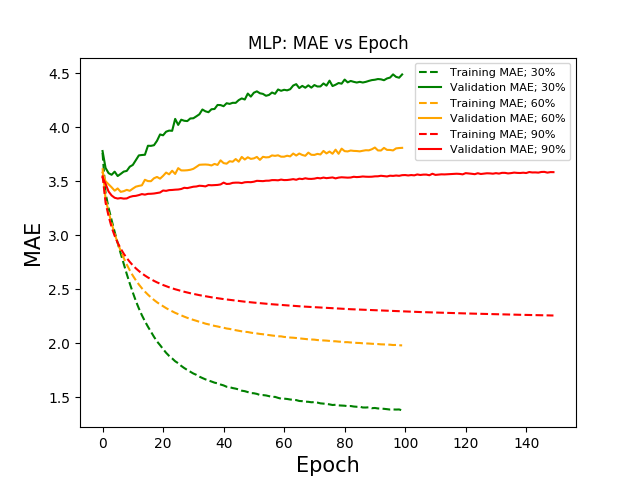
\includegraphics[width=0.9\textwidth]{mlp_mae.png}
        \end{center}

        \quad For a pair of training and validation sets, the validation MAEs are computed after each epoch is finished, but the training MAEs are taken directly from \texttt{keras.models.Model.fit()} which is the mean of all MAEs calculated after each batch during an epoch of training. Although the sizes of the training set across different pairs are identical, the sizes of validation sets are not. Therefore, validation MAE of each pair is multiplied by a constant $c_i$ before summation where $c_i=size(val\_set_i) / 30,000$ and $i$ is the index of the pair, which is just a linear combination of constants $c_i$ and the absolute error matrix and can be computed by finding

        \[
        \begin{bmatrix}
          MAE_1 & MAE_2 & \dots & MAE_n
        \end{bmatrix}
        =
        \begin{bmatrix}
          c_1 & c_2 & \dots & c_p \\
        \end{bmatrix}
        \times
        \begin{bmatrix}
          E_1^{(1)} & E_2^{(1)} & \dots  & E_n^{(1)} \\
          E_1^{(2)} & E_2^{(2)} & \dots  & E_n^{(2)} \\
          \vdots    & \vdots    & \vdots & \vdots \\
          E_1^{(p)} & E_2^{(p)} & \dots  & E_n^{(p)}
        \end{bmatrix}
        \]

        where $p$ denotes the total number of pairs, $n$ denotes the total number of epochs, $E_j^{(i)}$ denotes the absolute error of pair $i$ at epoch $j$.


      \newpage\subsection{Ternary Comparison}

        \begin{center}
          \textit{Proportion of each ternary with each training size's optimal rank or epoch.}

          \begin{tabular}{| c || c| c | c|}
            \hline
            &\multicolumn{3}{c|}{Ternary Proportion} \\
            \hline
            Model & a & b & c \\
            \hline
            NMF (90\%) & 55.300\%  & 29.640\% & 15.060\% \\
            NMF (60\%) & 54.523\%  & 29.647\% & 15.830\% \\
            NMF (30\%) & 51.253\%  & 30.703\% & 18.043\% \\
            \hline
            MLP (90\%) & 54.813\%  & 29.333\% & 15.853\% \\
            MLP (60\%) & 53.760\%  & 29.967\% & 16.273\% \\
            MLP (30\%) & 52.373\%  & 29.280\% & 18.347\% \\
            \hline
            Total Average & 14.257\% & 11.180\% & 74.563\% \\
            Uniformly Random & 12.720\% & 13.560\% & 73.720\% \\
            User Average &  8.463\% & 12.283\% & 79.253\% \\
            \hline
          \end{tabular}

          \textit{Note: a: MAE $\in (-\infty ,3)$; b: MAE $\in [3 ,6)$; c: MAE $\in [6 ,\infty)$.}

        \end{center}


\newpage \section*{References}

\small

[1]	Xiangnan He, Lizi Liao, Hanwang Zhang, Liqiang Nie, Xia Hu, Tat-Seng Chua. Neural Collaborative Filtering. \textit{arXiv preprint arXiv:1708.05031}


[2] Yoshua Bengio, Rejean Ducharme, Pascal Vincent. A Neural Probabilistic Language Model (2001).


[3] Xiang Li, Shuo Chen, Xiaolin Hu, Jian Yang. Understanding the Disharmony between Dropout and Batch Normalization by Variance Shift. \textit{arXiv preprint arXiv:1801.05134}

\end{document}